\chapter{System Description}
\label{sec:SystemDescription}

In this chapter, first will be a short analysis of the markers used in this project, the Apriltags. Then will be presented some information about the MAV, used to conduct experiments both in simulation and in real world. And finally there will be the system's coordinate frame analysis.

\section{Apriltags}
\label{sec:apriltags} 

In this project, the markers used to provide visual commands to the MAV were the Apriltags. They were created by Edwin Olson at the university of Michigan. These are visual fiducials, that mean artificial landmarks easily recognizable and distinguishable from one another. In contrast with other similar systems, they provide low volume of information, usually between 4 till 12 bits, thus they don't need high resolution images which allows long detection ranges. They differ from other similar approaches because they provide robustly 6 DOF position estimation while they can be printed with a standard printer and they can still provide detection under variable lighting conditions or even deformation of the paper on which they are printed. They have been widely used to provide ground truth trajectories in structured environments, Simultaneous Localization And Mapping (SLAM) and they are very common in augmented reality applications \cite{olson2011tags}.

\begin{figure}
   \centering
   
\includegraphics[width=0.55\textwidth]{images/tag36h11_im_large.pdf}
   \caption{The first Apriltag (id=0) of the tag36h11 family}
   \label{pics:tag36h11}
\end{figure}
 
There are various families of Apriltags, providing a large number of different markers. In figure \ref{pics:tag36h11} is presented the first aprliltag (id = 0) of the most common apriltag family, the "tag36h11". The aforementioned family, is the one suggested for use by the authors, and is also the default choice in the given detection algorithm. The difference between these families of markers is located at the amount of information carried by each tag.

As it can be easily seen by the aforementioned, the Apriltags were selected for use in this project for three main reasons. First, we wanted to use only detection data provided by the MAV's onboard camera. They provide robust position estimate and robust detection, by tolerating lighting variations and physical deformation of the marker. 


\section{AscTec Firefly}
\label{sec:ascTecFirefly}

The AscTec's Firefly MAV was used both in the simulated and in the real experiments. This particular MAV, is a hexacopter, thus it has six rotors that provide a stable flight. It is equipped with a powerful Intel$^{\circledR}$ Core$^{TM}$ i7 processor, that allows us to run ROS along with all the visual tracking algorithms onboard, without significant time delays.

In our specific case the MAV was equipped with the Skybotix's VI (Visual Inertial) sensor \cite{Nklc2014}. The sensor is equipped with two cameras and an IMU unit. In our experiments only one camera was used in order to identify the Apriltags and localize against them. It should be mentioned, that the MAV with the aforementioned sensor are modeled into the RotorS simulator.

\begin{figure}
   \centering
   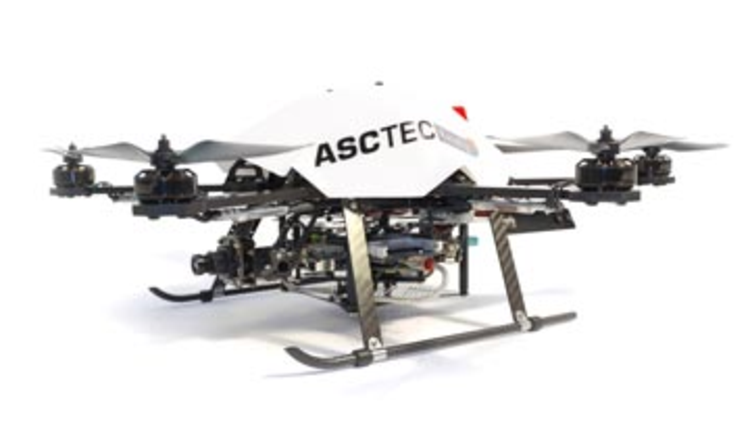
\includegraphics[width=0.55\textwidth]{images/AscTecFirefly.pdf}
   \caption{The Firefly MAV\protect\footnotemark}
   \label{pics:tag36h11}
\end{figure}
\footnotetext{The Firefly's image was taken from http://www.asctec.de/en}  
 

\section{Coordinate Frames}
\label{sec:CoordianteFrames}

A very crucial part of this project, was the analysis of the MAV's coordinate systems. This is very important because the MAV detects its desired position from  its camera detections and then has to transform these detections, from the camera frame to the controller's reference frame with respect to the world frame. Furthermore, the Apriltag's position in the simulated world is defined by it's pose as detected from the usb camera. Thus, by correctly defining and analyzing the coordinate frames we will be able to correctly interpret the position data from the marker detection and also apply the safety distances, so as to achieve our goals to move the MAV based on the detections of the Apriltags and also keep a safety distance between itself and the marker. For the transformations the ASL's minkindr library was used. It should be noted, that the color coding in the axes frames follows the RVIZ color convention, meaning red depicts the x-axis, green the y-axis and blue the z-axis respectively. Furthermore the ASL's frame naming convention \cite{FrameNamingConvention} is followed throughout this project. 

\subsection{Coordinate Frames in the Simulation }
\label{sec: CoordinatesinSimulation}
 
The first thing that should be resolved in the simulation world, was the correct positioning of the apriltag with respect to the usb camera detection. Although the two frames share the same origin point, the have different orientations as seen by figure \ref{pics:worldcamframe}, the distance between the two frames is set to emphasize the rotation. As it can be seen the transformation form camera frame with respect to the world frame, $R_{W\textunderscore USBC}$, consists of one rotation of $90^{\circ}$ around the y-axis $(Rot_{y}(90^{\circ}))$ and a successive rotation of $-90^{\circ}$ around the z-axis $(Rot_z(-90^{\circ}))$ as presented in the equation \ref{eq:camtoworldrot}. With the aforementioned transformation, the coordinates as seen from the camera match the actual world coordinates. 
 
\begin{equation}
\label{eq:camtoworldrot}
\left[\begin{array}{c}
x_{wc} \\ y_{wc} \\ z_{wc}  \end{array} \right] = Rot_{y}(90^{\circ})Rot_z(-90^{\circ})\left[ \begin{array}{c} x_c \\ y_c \\z_c \end{array} \right]
\end{equation}
 
  
\begin{figure}
  \centering
  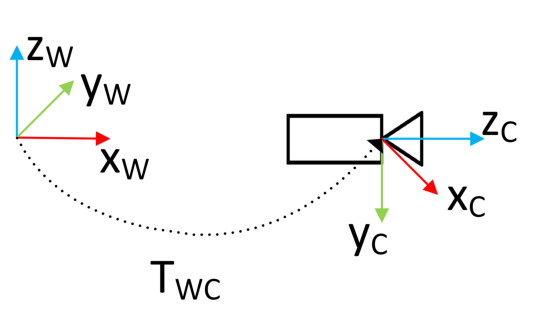
\includegraphics[width=0.98\textwidth]{images/world_cam_v2.pdf}
  \caption{The image represents the world coordinate frame and the camera frame.}
  \label{pics:worldcamframe}
\end{figure}
 
After the transformation of the camera frame, now come the coordinate transformations regarding the MAV. The transformation between the MAV's body frame and the world frame is obtained by the firefly's odometry sensor, in the simulation it is named as odometry\textunderscore sensor1, the obtained transformation is represented by $T_{W\textunderscore B}$. This transformation reveals the real pose of the MAV in the world reference frame, as it is perceived from its IMU sensor. Then the static transform between the body frame and the onboard camera frame is provided as parameter by the configuration file and is represented as $T_{B\textunderscore C}$. The aforementioned transform is passed as parameter in order to reduce the calculations needed to be perform and thus, speed up the procedure. The transformation between the MAV's camera and the Apriltag is obtained by the detection algorithm, by subscribing to the MAV's  tag\textunderscore detection\textunderscore pose topic. This provides the pose of the detected Apriltag with respect to the camera coordinate frame. The last part was to obtain the transformation between the Apriltag frame and the reference frame. It is  easily understood, that this is the most crucial part since it defines the desired coordinates towards which, we command the MAV to move to. As it can be seen from the \ref{pics:mavcoordinateframe} the reference frame has the same orientation as the world system and is translated from it by the offsets specified by the user in the parameters' file. The transformation between the apriltag frame with respect to the reference frame can be seen from the image \ref{pics:mavcoordinateframe}, while the rotation is composed by a rotation around the y-axis by $-90^{\circ}$ and a rotation around the z-axis by $90^{\circ}$.The offsets, and especially the offset in the x-axis since this defines the straight distance between the MAV and the Tag, are added so as to ensure that the MAV will keep a safety distance between itself, the Apriltag and the user holding it. If the x offset is set to zero, then the reference frame coincides with the Tag's frame, and they will collide, since the reference position of the MAV is set to the exact equal coordinates of the Tag. The aforementioned are presented in matrix \ref{matrix:TRA}, of course $T_{R\textunderscore A}$ is a 4 x 4 homogeneous transformation presented in matrix \ref{matrix:TRA}. The final coordinates that are sent to the controller are the result of the transformation presented in equation \ref{TWR} and they express in the coordinates at the reference frame with respect to the world frame.
 

\begin{table}
$$
\renewcommand{\arraystretch}{2}
\newcommand*{\temp}{\multicolumn{1}{c|}{}}
T_{R\textunderscore A} = \left[\begin{array}{c|c}
Rot_y(-90^{\circ}) * Rot_z(90^{\circ}) & offset\textunderscore x \\ &offset\textunderscore y \\ &offset\textunderscore z \\ \hline
\overrightarrow{0} & 1
\end{array}\right]
$$
\caption{The transformation from Apriltag to Reference frame}
\label{matrix:TRA}
\end{table}
 
 
\begin{equation}
\label{TWR}
T_{W\textunderscore R} = T_{W\textunderscore B} * T_{B\textunderscore C} * T_{C\textunderscore A} * {T_{R\textunderscore A}}^{-1}
\end{equation}  
 
\begin{figure}
 \centering
 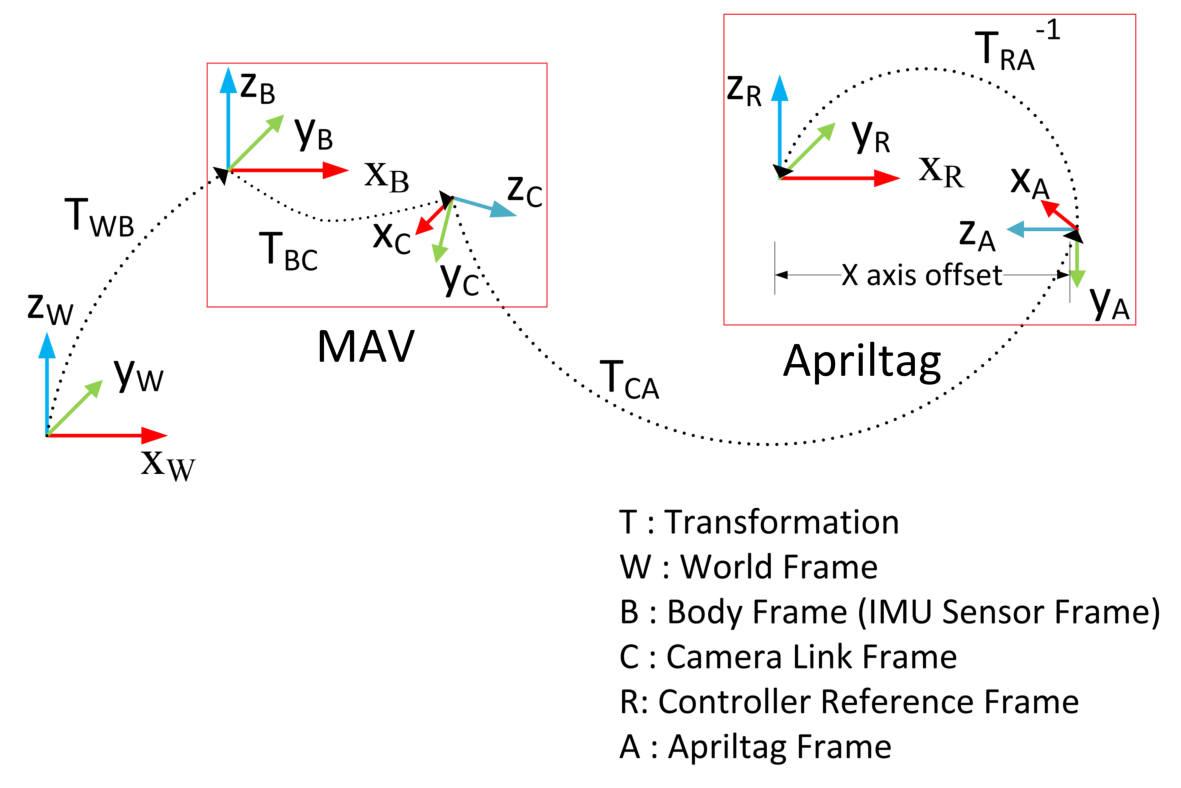
\includegraphics[width=0.99\textwidth]{images/coordinate_frame_representation_v3b.pdf}
 \caption{The MAV detects the Apriltags coordinates with respect to its camera frame. The appropriate transformations are made to transform the apriltag coordinates to the reference frame with respect to the world frame. In the controller reference frame the safety offsets are added so as to ensure that a collision between the MAV and the marker is avoided.}
 \label{pics:mavcoordinateframe}
\end{figure}
  
  
\subsection{Coordinate Frames in the Real System}
\label{sec: CoordinatesinRealSystem}
  
In the real system the coordinate frames are as expected the same, with minor numerical differences. These numerical differences were expected since it is not possible to have a "perfect" recreation of the real system in the simulation. 

